\section{CNN from Scratch}
This chapter shows the results of the training of several custom architecture, that have been defined in order to solve the classification task.
Starting from a very simple model, we start to analyze how to improve it and what modifications to apply in order to improve performance, taking into account mainly the accuracy on the validation test, but also considering other metrics like training time or number of parameters.
The overall strategy is the following:
\begin{itemize}
\item test of different custom architectures defined from scratch
\item analysis of the level of fitting, try of different techniques to fight possible underfitting/overfitting
\item experiment with the addition of Batch Normalization
\item hyperparameters optimization on the best model so far
\end{itemize}

The objective of the presented procedure is not the total exploration and exploitation of the search space, but it aims at finding good results in a reasonable time exploiting an ad-hoc heuristic search.
The tested models are the following:

\subsection{Standard CNN}
\subsubsection{Simple model}
The first experiment has been conducted using a customized standard CNN that exploits Convolutional Layers and Max Pooling to process input images. To start, we defined a very simple model, whose structure is reported in the image \ref{fig:standardCNN}. This network is mainly a starting point of our trial-and-error approach and will give us a first approximation of what is going to be our prediction power on the considered task.
\begin{figure}[H]
	\centering
	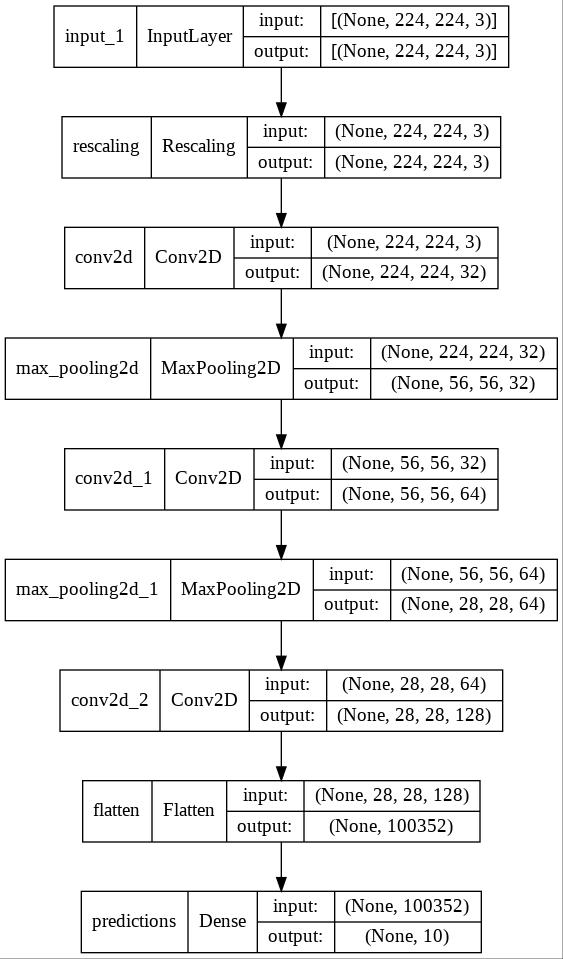
\includegraphics[height=0.6\textwidth]{img/scratch/standardCNN.jpg}
	\caption{Customized Standard CNN Architecture}
	\label{fig:standardCNN}
\end{figure}

\noindent This model is trained using these default hyperparameters:
\begin{itemize}
\item optimizer: \textit{ADAM}
\item dropout rate: 0.0
\item learning rate: optimizer's default
\item batch size: 128
\item learning rate decay: optimizer's default
\end{itemize}

\noindent In particular, we set a large value for batch size both because our main goal is to maximize the accuracy and also (as presented in the \textit{Introduction}) to face off with the great variability of paintings with very dissimilar style but belonging to the same author. In this way, we increase the probability of a batch to be "complete", thus being representative of this variability.

\noindent The results obtained are the following:

\medskip

\begin{tabular}{ |p{2cm}|p{2cm}|p{2cm}|p{2cm}|p{2cm}|  }
\hline
\multicolumn{5}{|c|}{StandardCNN} \\
\hline
\textbf{Epoch stopped} & \textbf{Validation Accuracy} & \textbf{Test Accuracy} & \textbf{Validation Loss} & \textbf{Test Loss} \\
\hline
15 & 0.5730 & 0.786 & 1,3656 & 0.6542\\
\hline
\end{tabular}

\medskip


\begin{figure}[H]
	\begin{subfigure}{0.5\textwidth}
		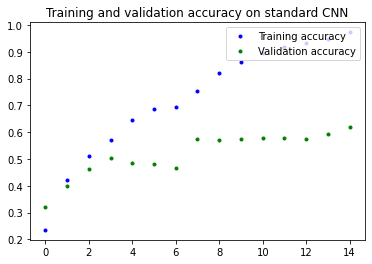
\includegraphics[width=0.9\linewidth]{img/scratch/standardCNN_results_accuracy.png} 
		\caption{Standard CNN Accuracy}
		\label{fig:standardCNNacc}
	\end{subfigure}
	\begin{subfigure}{0.5\textwidth}
		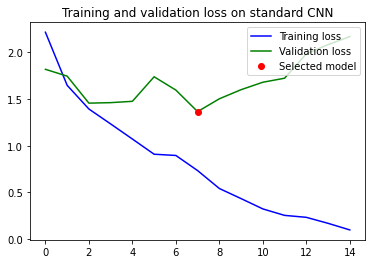
\includegraphics[width=0.9\linewidth]{img/scratch/standardCNN_results_loss.png}
		\caption{Standard CNN Loss}
		\label{fig:standardCNNloss}
	\end{subfigure}
\end{figure}

\medskip

\noindent The result on test set is stunning, however we believe that it has been a lucky coincidence more than an actual prediction power, given the fact that the relative training and validation accuracy were respectively 0.68 and 0.57. Both the discrepancy between validation and test accuracy and the fact that 79\% is actually higher than training accuracy prove that this value is just a happy coincidence, probably given a high similarity between the training samples correctly learned by the network and the test samples. The maximum validation accuracy value is equal to 57.3\% and it is reached in just 8 epochs, then the network overfits very quickly. It can be caused by mainly 3 factors:
\begin{itemize}
\item Data available is insufficient, so the network loses the ability to generalize
\item Lack of regularization techniques, such as Dropout or L1/L2 regularizations
\item \textbf{The spatial extent of the feature map of the last layer is still quite large, so the fully connected layers have too many parameters operating in a quite shallow representation.} 
\end{itemize} 

\subsubsection{Deeper network and dropout}
The highlighted problem can be tackled exploiting a deeper architecture, in which we add more convolutional layers in order to reduce the spatial extent of the extracted features, together with the reduction of parameters and the further processing applied to the original image: in this way we expect the network to have higher capacity and to need more epochs to overfit, thus incrementing accuracy.
To better process the feature vector, we also added a 32-neurons \textit{Fully-Connected }layer, right before the \textit{Softmax} classifier. In order to avoid overfitting that could be caused by those additional parameters we introduce \textit{Dropout} regularization to the latter layer.   
The final resulting network is the one reported in the figure below\ref{fig: DeeperDropout}.

\begin{figure}[H]
	\centering
	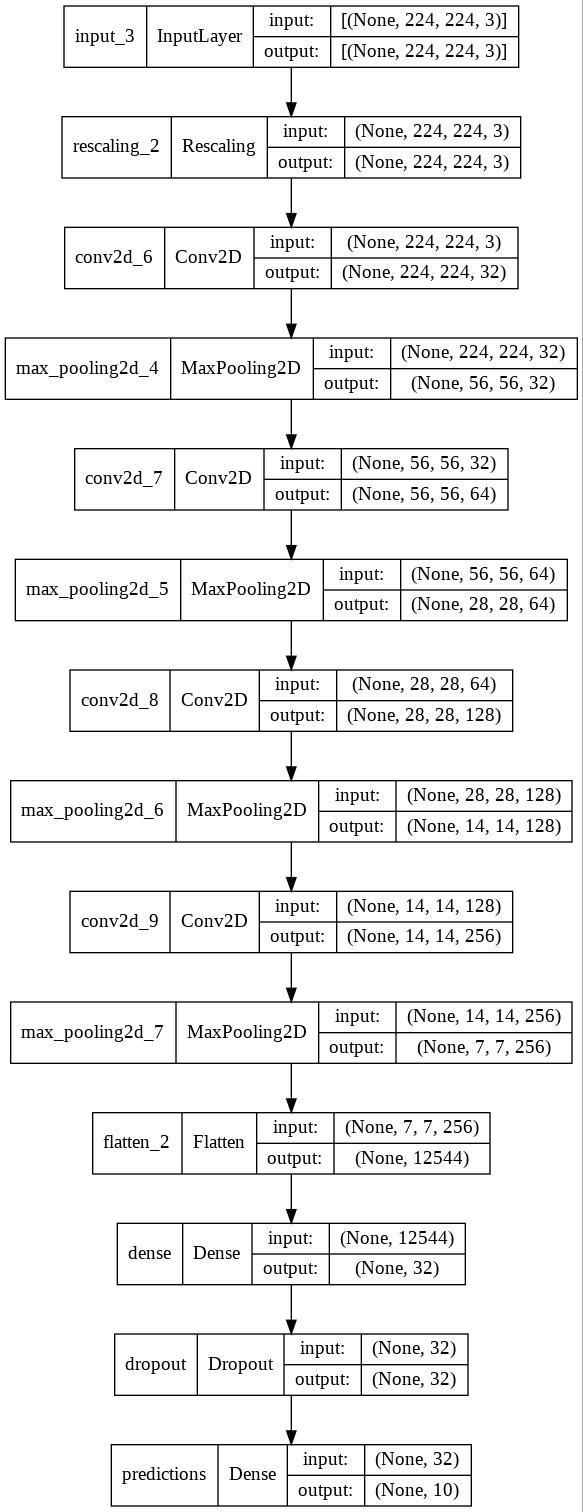
\includegraphics[height=0.8\textwidth]{img/scratch/DropoutCNN.jpg}
	\caption{Deeper CNN with Dropout Architecture}
	\label{fig: DeeperDropout}
\end{figure}

\noindent Again, we train the network for at least 15 epochs. To optimize the training process, we actually tune dynamically the number of epochs and we save the history of the training itself. In this way we can interrupt and restart the learning phase, visualize the intermediate results and save in an external file the model that, during training, achieved best validation accuracy. Whenever possible, we train the network till the convergence of training loss, thus visualizing when and how fast the model started to overfit and trying to understand what can be the causes.

\noindent The results obtained are the following:

\medskip

\begin{tabular}{ |p{2cm}|p{2cm}|p{2cm}|p{2cm}|p{2cm}|  }
\hline
\multicolumn{5}{|c|}{Deeper CNN with Dropout} \\
\hline
\textbf{Epoch stopped} & \textbf{Validation Accuracy} & \textbf{Test Accuracy} & \textbf{Validation Loss} & \textbf{Test Loss} \\
\hline
45 & 0.590 & 0.6244 & 1.1996 & 1.1516\\
\hline
\end{tabular}

\medskip


\begin{figure}[H]
	\begin{subfigure}{0.5\textwidth}
		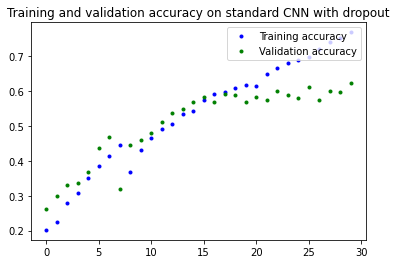
\includegraphics[width=0.9\linewidth]{img/scratch/deeper_dropout_acc.png} 
		\caption{Deeper CNN with Dropout accuracy}
		\label{fig:DeeperDroupoutacc}
	\end{subfigure}
	\begin{subfigure}{0.5\textwidth}
		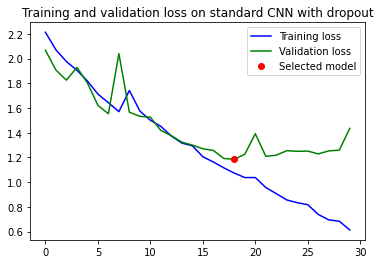
\includegraphics[width=0.9\linewidth]{img/scratch/deeper_dropout_loss.png}
		\caption{Deeper CNN with Dropout loss}
		\label{fig:DeeperDropoutloss}
	\end{subfigure}
\end{figure}

\medskip

\noindent Analyzing these graphs, we realize that the validation accuracy is actually improved, and also test accuracy and loss are coherent with validation ones. The increased network capacity improved its ability to generalize, but we now have a problem, that is the model couldn't converge (not shown in the graphs above), starting to oscillate once reached 1.2 of training loss. We can argue that is due a too high learning rate value, but we actually use ADAM as optimizer which is able to dynamically tune it to proceed with learning. Thus the cause could be the underfitting: since we deepened the network, we are providing the few dense neurons with a feature vectors whose variability is now much bigger than before as result of the further processing. The phenomenon is exacerbated by the Dropout, that reduces Fully-Connected capacity by 20\% at each epoch. If we could train further, we might have found a model that also improves validation accuracy.



\subsubsection{Bigger Network and Early Stopping}
If the problem is the overfitting, we can try to go further and increase network dimensions at FC layers. With this experiment we apply that, expecting to see our network to converge. If our hypothesis is correct, we expect the accuracy value to be more or less the same or at least to increase, while if it is not, we expect the validation loss to diverge quickly. The network we are going to test is the following\ref{fig:BiggerCNN}:

\begin{figure}[H]
	\centering
	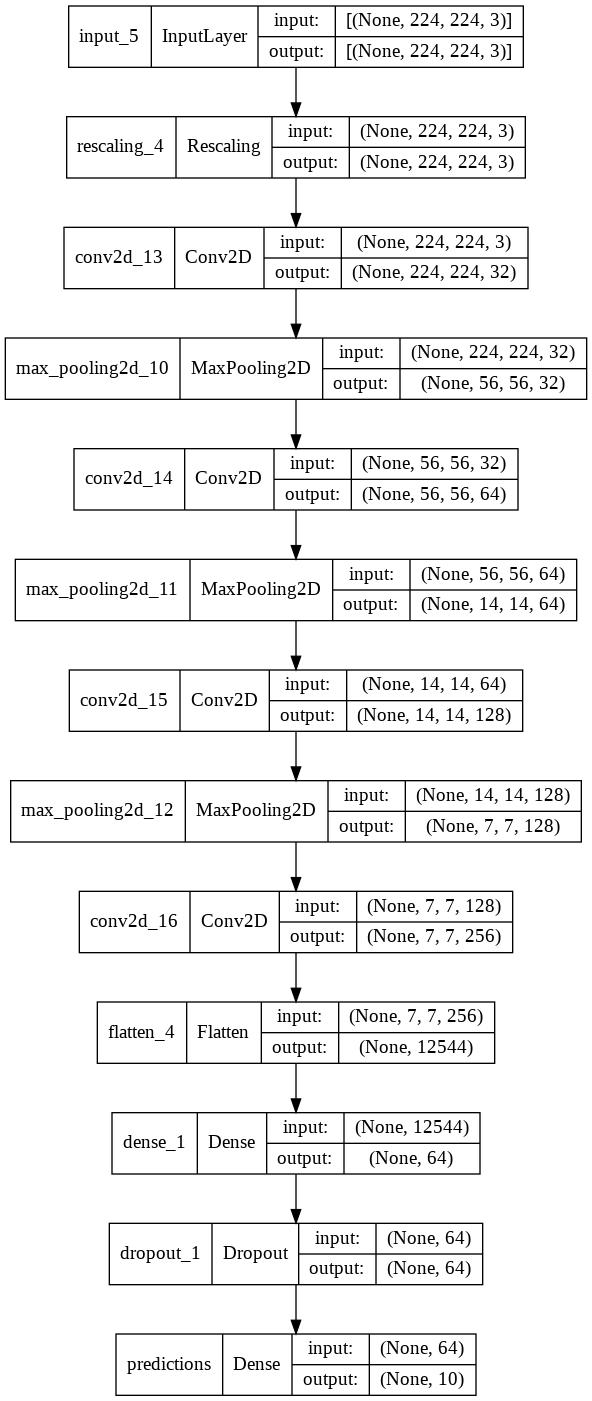
\includegraphics[height=0.8\textwidth]{img/scratch/BiggerCNN.jpg}
	\caption{Customized architecture with bigger FC layers}
	\label{fig:BiggerCNN}
\end{figure}

\noindent This time we introduced the \textit{Early Stopping} to the training process: Early Stopping is a mechanism offered by Keras among the possible callbacks, that consist on halting the training process if some condition is fired. In our case we monitor the validation loss (not the accuracy, the primer is more robust since it takes into account also class weights and how much a network is confident on its classification, while the latter only considers the number of correctly classified samples), whenever the model does not improve it for a certain number of epochs (patience value), training process is stopped. Thanks to the previously explained mechanism, we are still able to resume it manually if we believe that the validation values may actually improve.

\noindent The outcome of the learning is the following:

\medskip

\begin{tabular}{ |p{2cm}|p{2cm}|p{2cm}|p{2cm}|p{2cm}|  }
\hline
\multicolumn{5}{|c|}{Bigger CNN} \\
\hline
\textbf{Epoch stopped} & \textbf{Validation Accuracy} & \textbf{Test Accuracy} & \textbf{Validation Loss} & \textbf{Test Loss} \\
\hline
30 & 0.638 & 0.6443 & 1.1321 & 1.1742\\
\hline
\end{tabular}

\medskip


\begin{figure}[H]
	\begin{subfigure}{0.5\textwidth}
		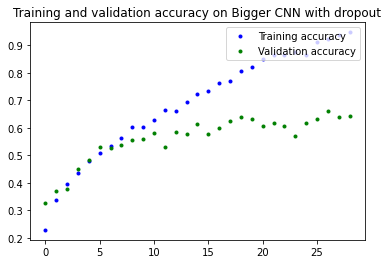
\includegraphics[width=0.9\linewidth]{img/scratch/bigger_acc.png} 
		\caption{Bigger network accuracy}
		\label{fig:BiggerCNNacc}
	\end{subfigure}
	\begin{subfigure}{0.5\textwidth}
		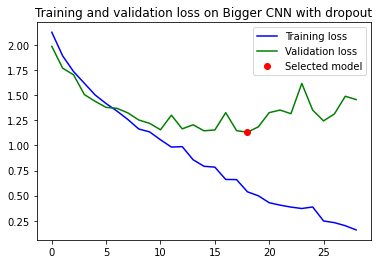
\includegraphics[width=0.9\linewidth]{img/scratch/bigger_loss.png}
		\caption{Bigger network loss}
		\label{fig:BiggerCNNloss}
	\end{subfigure}
\end{figure}

\medskip

\noindent Accuracy and loss are actually improved, and the convergence problem is now solved. Increasing capacity but equipping the network with the Dropout regularization allowed it to increase its learning power, but avoiding neurons to overspecialize themselves, and this had a beneficial effect on the architecture.

\subsubsection{Batch Normalization}
The previous model showed quite good results, however we wonder if we can improve it. For this purpose we try to use the \textit{Batch Normalization}.
Batch Normalization is a technique that is frequently used to make the training process more stable, usually gaining also better accuracies especially on very big and deep networks. Batch normalization is not formally proved, but the idea is quite simple: given a batch of input training samples, we subtract each by their mean and divide them by their standard deviation, thus obtaining a Gaussian Normal distribution of the inputs. To give an oversimplified view of the intuition, given a 2d linearly-separable dataset and a linear activation, to find the best dividing straight is much easier if all the points are near the origin rather than if they are far away: the found line will be much more robust. Batch Normalization tries to apply such transformation to all the samples of each batch, and it's usually exploited right before the non-linear activation (ReLU in our case). At test time, BN parameters are not computed on the test batch, but the average training ones are used. Taking as base the previous network (Bigger CNN), which is the one that performed best so far, and adding the Batch Normalization layers we obtain the following architecture:\ref{fig: BatchNormalizationCNN}

\begin{figure}[H]
	\centering
	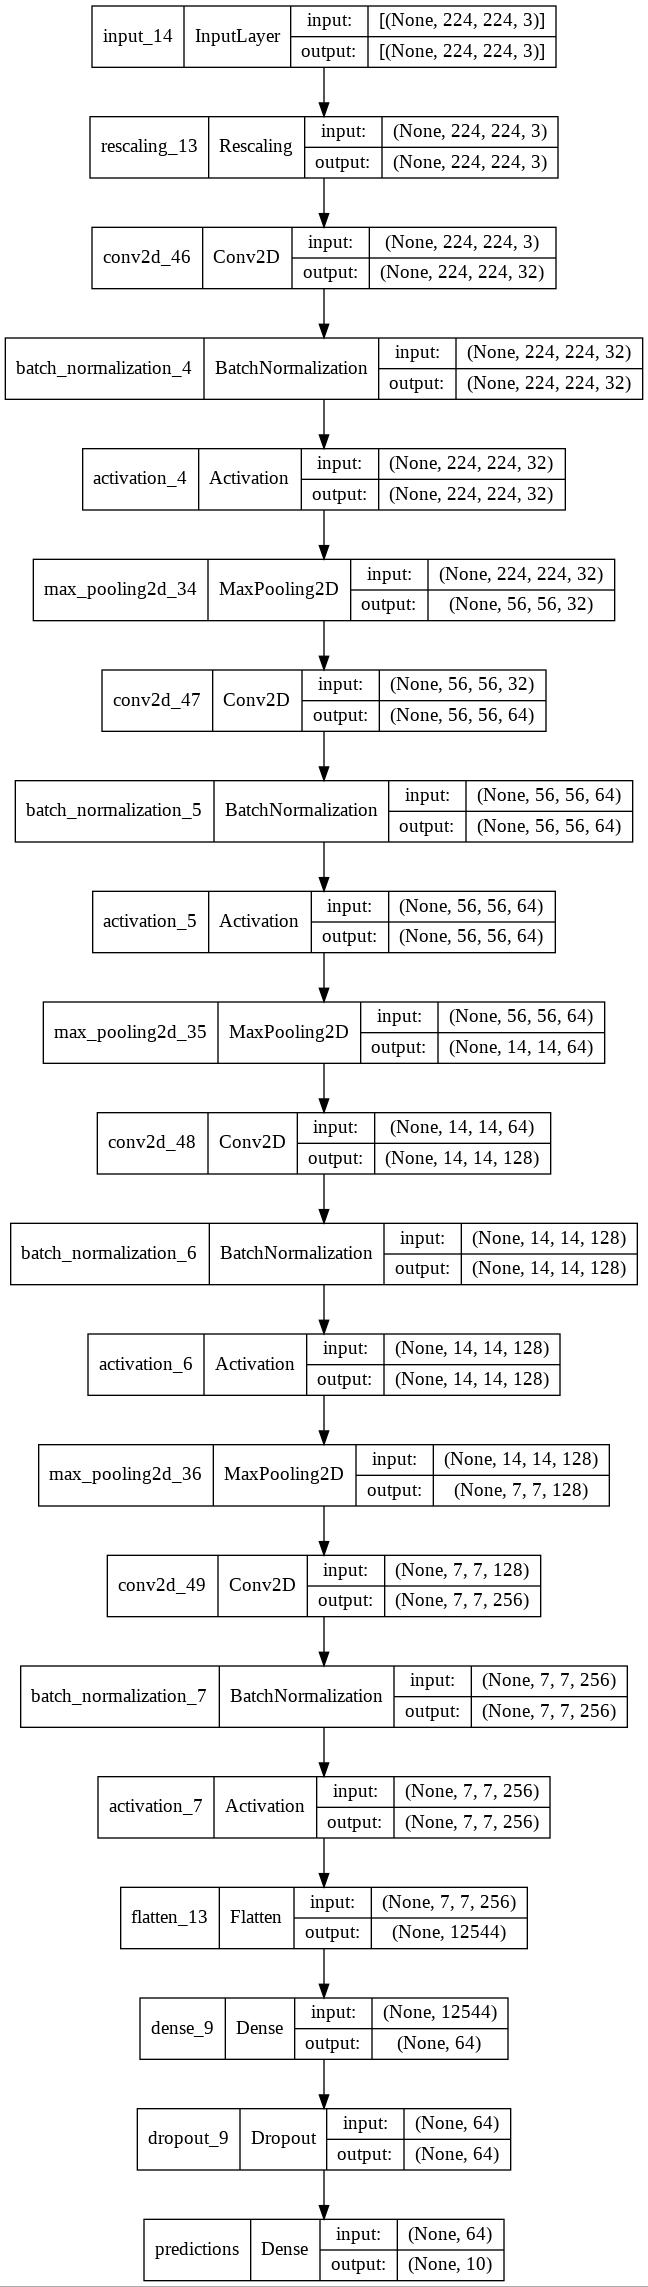
\includegraphics[height=1.4\textwidth]{img/scratch/batch_normalization.jpg}
	\caption{CNN architecture with batch normalization}
	\label{fig: BatchNormalizationCNN}
\end{figure}

\noindent This figure could be a little bit misleading because, once separated activations from Convolutional Layers, the network seems to be deeper. Actually it is not.

\noindent The results of the training process are: 

\medskip

\begin{tabular}{ |p{2cm}|p{2cm}|p{2cm}|p{2cm}|p{2cm}|  }
\hline
\multicolumn{5}{|c|}{CNN with Batch Normalization} \\
\hline
\textbf{Epoch stopped} & \textbf{Validation Accuracy} & \textbf{Test Accuracy} & \textbf{Validation Loss} & \textbf{Test Loss} \\
\hline
35 & 0.604 & 0.6144 & 1.1978 & 1.2942\\
\hline
\end{tabular}

\medskip


\begin{figure}[H]
	\begin{subfigure}{0.5\textwidth}
		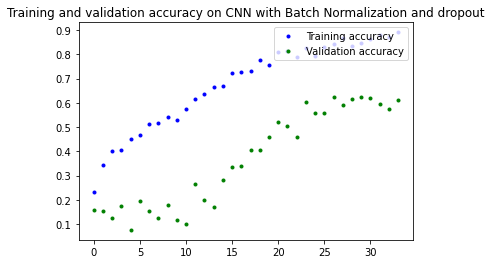
\includegraphics[width=0.9\linewidth]{img/scratch/batch_normalization_acc.png} 
		\caption{Bigger CNN with Batch Normalization accuracy}
		\label{fig:BatchNormalizationacc}
	\end{subfigure}
	\begin{subfigure}{0.5\textwidth}
		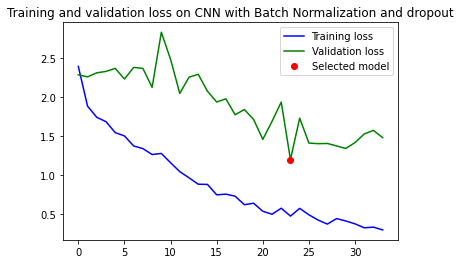
\includegraphics[width=0.9\linewidth]{img/scratch/batch_normalization_loss.png}
		\caption{Bigger CNN with Batch Normalization loss}
		\label{fig:BatchNormalizationloss}
	\end{subfigure}
\end{figure}

\medskip

\noindent Batch Normalization is very useful for big networks, however it showed no improvement in our experiment, adding noise to the learning process. This is also due to the limited number of training examples: mean and standard deviation are not very representative of the whole application domain, so they could differ very much from the ones of validation or test set


\subsubsection{Data Augmentation}
Last experiment conducted on standard CNNs exploits Data Augmentation. Data Augmentation is a techinique that consists on artificially expanding labeled training dataset by applying affine transformation or elastic deformations\footnote{PEREZ, Luis; WANG, Jason. The effectiveness of data augmentation in image classification using deep learning. arXiv preprint arXiv:1712.04621, 2017.}. The idea is to try to increase accuracy by reducing more the overfitting, and it could be particularly suitable in our case where we have a very small dataset with several classes. In the following, we apply data augmentation to the model that performed best so far (paragraph 3.1.3)\ref{fig: DataAugmentationStandardCNN}.

\begin{figure}[H]
	\centering
	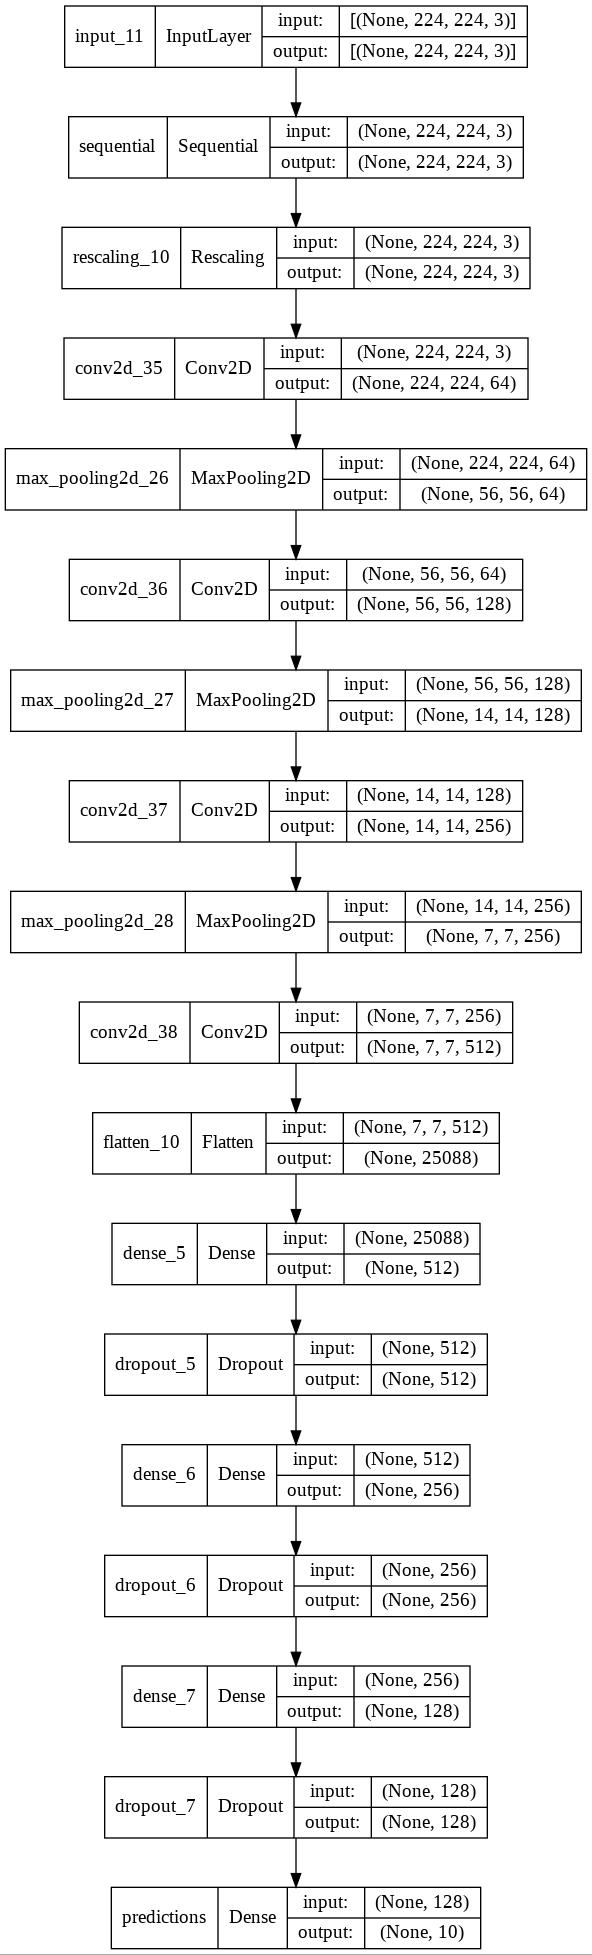
\includegraphics[height=1.2\textwidth]{img/scratch/DataAugmentedCNN.jpg}
	\caption{CNN architecture with data augmentation}
	\label{fig: DataAugmentationStandardCNN}
\end{figure}

\noindent The results of the training process are: 

\medskip

\begin{tabular}{ |p{2cm}|p{2cm}|p{2cm}|p{2cm}|p{2cm}|  }
\hline
\multicolumn{5}{|c|}{CNN with Data Augmentation} \\
\hline
\textbf{Epoch stopped} & \textbf{Validation Accuracy} & \textbf{Test Accuracy} & \textbf{Validation Loss} & \textbf{Test Loss} \\
\hline
31 & 0.360 & 0.4055 & 1.8218 & 1.7557\\
\hline
\end{tabular}

\medskip


\begin{figure}[H]
	\begin{subfigure}{0.5\textwidth}
		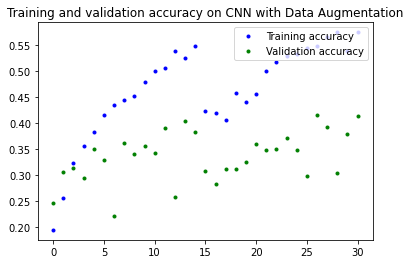
\includegraphics[width=0.9\linewidth]{img/scratch/data_augmentation_acc.png} 
		\caption{Bigger CNN with Data Augmentation accuracy}
		\label{fig:DataAugmentationacc}
	\end{subfigure}
	\begin{subfigure}{0.5\textwidth}
		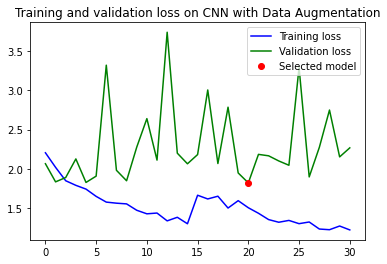
\includegraphics[width=0.9\linewidth]{img/scratch/data_augmentation_loss.png}
		\caption{Bigger CNN with Data Augmentatio loss}
		\label{fig:DataAugmentationloss}
	\end{subfigure}
\end{figure}

\medskip

\noindent The training process is very very noisy and the model severely underfits. The noise can be explained by the high randomness amount that has been inserted in the learning process, both due to droupout and the random transformations of data augmentation itself.
The underfitting was actually predictable: data augmentation is used mainly to contrast overfitting, but the 3.1.3 model actually overfitted very late.
The only solution would be the training of a larger, deeper network, thus increasing parameters that can be trained and reducing overfitting: we tried such approach and it was actually promising, however Colab limitations halted the training and we concluded that it was impossible to train such a big model from scratch.


\subsection{Aggressive Downsampling}
Aggressive Downsampling consists on designing a Convolutional neural network such that, first of all, it shrinks very rapidly the spatial extent of the input image: in this way the number of initial parameters are drastically reduced, allowing for deeper networks and more FC layers. The idea is that in the input image (especialy for high-resolution ones), contiguous pixels have similar values, so even such an aggressive initial downsampling does not destroy much information. GoogleNet and AlexNet are examples of networks exploiting Aggressive Downsampling. In the following section, we define and train some network with aggressive downsampling, comparing performance with the previous ones.

\subsubsection{Standard CNN with aggressive downsampling}
In this paragraph we analyze a model very similar to the 3.1.1 one, but it exploits aggressive downsampling. Thanks to that, the network is deeper but also has less parameters than the standard model, for sure reducing overtraining.
The architecture is the following\ref{fig: AggressiveDownsamplingCNN}:

\begin{figure}[H]
	\centering
	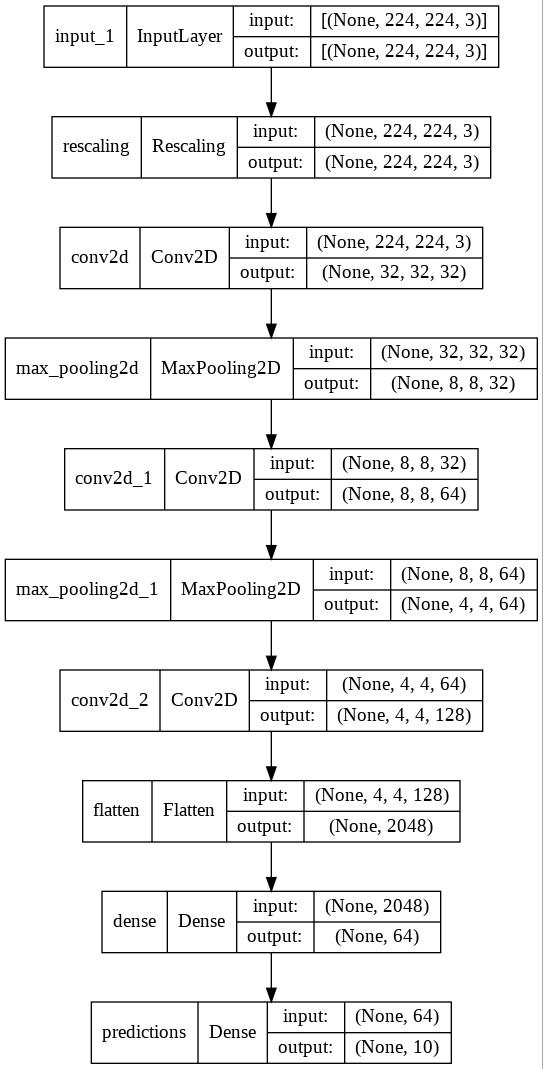
\includegraphics[height=0.8\textwidth]{img/scratch/aggressive_downsampling.jpg}
	\caption{standard CNN architecture with aggressive downsampling}
	\label{fig: AggressiveDownsamplingCNN}
\end{figure}

\noindent As we can observe, the number of parameters is reduced from more than 1 million to just 225 thousands, but despite this it has a fully connected layer more. The training process took much less computational time and the results are: 

\medskip

\begin{tabular}{ |p{2cm}|p{2cm}|p{2cm}|p{2cm}|p{2cm}|  }
\hline
\multicolumn{5}{|c|}{CNN with Aggressive Downsampling} \\
\hline
\textbf{Epoch stopped} & \textbf{Validation Accuracy} & \textbf{Test Accuracy} & \textbf{Validation Loss} & \textbf{Test Loss} \\
\hline
45 & 0.691 & 0.6194 & 1.0244 & 1.0796\\
\hline
\end{tabular}

\medskip


\begin{figure}[H]
	\begin{subfigure}{0.5\textwidth}
		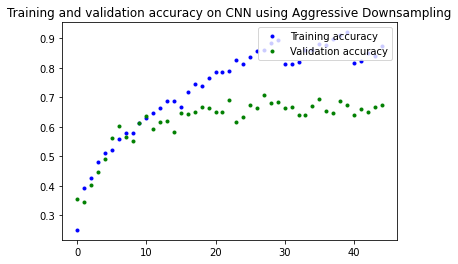
\includegraphics[width=0.9\linewidth]{img/scratch/aggressive_downsampling_acc.png} 
		\caption{CNN with aggressive downsampling accuracy}
		\label{fig:AggressiveDownsamplingacc}
	\end{subfigure}
	\begin{subfigure}{0.5\textwidth}
		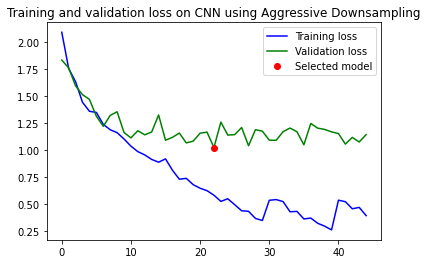
\includegraphics[width=0.9\linewidth]{img/scratch/aggressive_downsampling_loss.png}
		\caption{CNN with aggressive downsampling loss}
		\label{fig:AggressiveDownsamplingloss}
	\end{subfigure}
\end{figure}

\medskip

\noindent The choice of aggressive downsampling has sensational effects on the classification power of the network: with very few GPU memory consumed, this model outperforms the 3.1.1 one, especially on validation accuracy and loss. Since the test results of the standard CNN model were not reliable, we cannot compare them, but with respect to the other models presented in the section 3.1, this network has similar accuracy and better loss. The only problem came up around iteration 30: the network cannot converge but starts oscillating around the loss value of 0.5, also training accuracy oscillates while validation loss is stuck around 1.2.
The first hypothesis could be that the learning rate is too large in that training phase, but we used as optimizer Adam which computes individual adaptive learning rates for different parameters from estimates of first and second moments of the gradients, and its convergence is proved\footnote{KINGMA, Diederik P.; BA, Jimmy. Adam: A method for stochastic optimization. arXiv preprint arXiv:1412.6980, 2014.}, so the only possibility is that the network has too few parameters to learn all the train samples. In the following experiment we try to increase the network size to face such problem.


\subsubsection{Bigger CNN with aggressive downsampling}
As anticipated in the previous paragraph, in this experiment we test a bigger Convolutional NN that exploits aggressive downsampling, trying to solve the problem of missing convergence. Note that, even if it will be solved, it might not involve that validation and test accuracy will increase. The architecture is the following\ref{fig:BiggerAggressiveDownsamplingCNN}:

\begin{figure}[H]
	\centering
	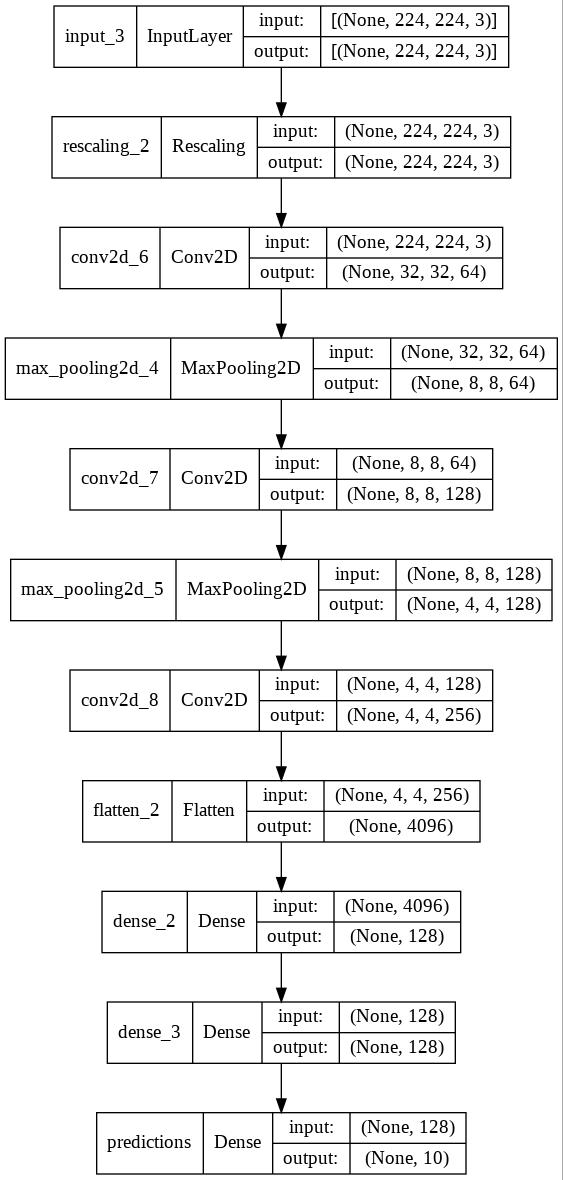
\includegraphics[height=1.0\textwidth]{img/scratch/bigger_aggressive_downsampling.jpg}
	\caption{Bigger CNN architecture with aggressive downsampling}
	\label{fig:BiggerAggressiveDownsamplingCNN}
\end{figure}

\noindent Number of parameters is much higher, almost 1 million. The training results are: 

\medskip

\begin{tabular}{ |p{2cm}|p{2cm}|p{2cm}|p{2cm}|p{2cm}|  }
\hline
\multicolumn{5}{|c|}{Bigger CNN with Aggressive Downsampling} \\
\hline
\textbf{Epoch stopped} & \textbf{Validation Accuracy} & \textbf{Test Accuracy} & \textbf{Validation Loss} & \textbf{Test Loss} \\
\hline
25 & 0.688 & 0.7910 & 1.0349 & 0.6340\\
\hline
\end{tabular}

\medskip


\begin{figure}[H]
	\begin{subfigure}{0.5\textwidth}
		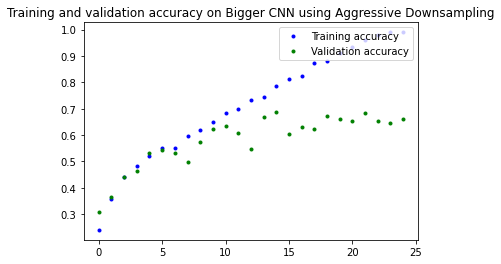
\includegraphics[width=0.9\linewidth]{img/scratch/bigger_ad_acc.png} 
		\caption{Bigger CNN with aggressive downsampling accuracy}
		\label{fig:BiggerAggressiveDownsamplingacc}
	\end{subfigure}
	\begin{subfigure}{0.5\textwidth}
		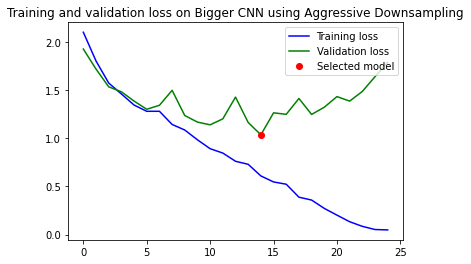
\includegraphics[width=0.9\linewidth]{img/scratch/bigger_ad_loss.png}
		\caption{Bigger CNN with aggressive downsampling loss}
		\label{fig:BiggerAggressiveDownsamplingloss}
	\end{subfigure}
\end{figure}

\medskip

\noindent Increasing parameters actually helped the network to reach convergence, and it showed comparable results on the validation test and great results on test set. However, as discussed in 3.1.1, it is very likely that with this random seed training and test set are quite more similar than training and validation ones, so the test metrics could be inflated by this fact.

\subsubsection{Bigger CNN with aggressive downsampling and data augmentation}
Despite the previous results, the graphs are still characteristics of overfitting: the best validation values where reached quite soon, and then they deteriorate quickly while the training loss continues to decrease. In this experiment we will try to fight overfitting introducing again data augmentation\ref{fig:dataAugmentedAggressiveDownsamplingCNN}:

\begin{figure}[H]
	\centering
	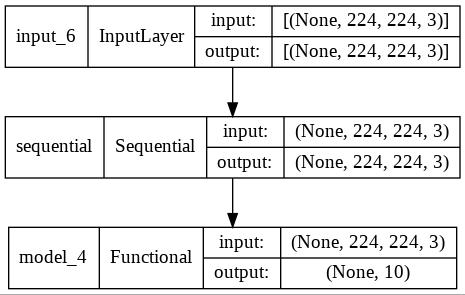
\includegraphics[height=0.4\textwidth]{img/scratch/DataAugmentedAggressiveDownsamplingCNN.jpg}
	\caption{Bigger CNN architecture with aggressive downsampling and data augmentation}
	\label{fig:dataAugmentedAggressiveDownsamplingCNN}
\end{figure}

\medskip

\noindent The central hidden model is the 3.2.2 one. Results of training are:

\medskip

\begin{tabular}{ |p{2cm}|p{2cm}|p{2cm}|p{2cm}|p{2cm}|  }
\hline
\multicolumn{5}{|c|}{Bigger CNN architecture with aggressive downsampling and data augmentation} \\
\hline
\textbf{Epoch stopped} & \textbf{Validation Accuracy} & \textbf{Test Accuracy} & \textbf{Validation Loss} & \textbf{Test Loss} \\
\hline
34 & 0.4803 & 0.5199 & 1.5720 & 1.4629\\
\hline
\end{tabular}

\medskip


\begin{figure}[H]
	\begin{subfigure}{0.5\textwidth}
		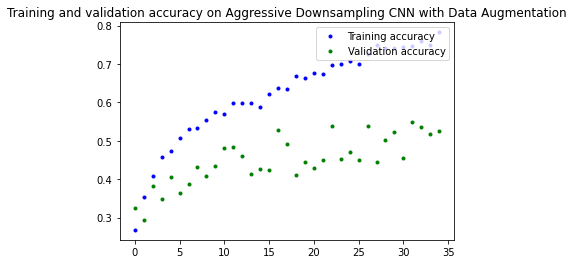
\includegraphics[width=0.9\linewidth]{img/scratch/data_augmented_ad_acc.png} 
		\caption{Bigger CNN with aggressive downsampling and data augmentation accuracy}
		\label{fig:DataAugmentedAggressiveDownsamplingacc}
	\end{subfigure}
	\begin{subfigure}{0.5\textwidth}
		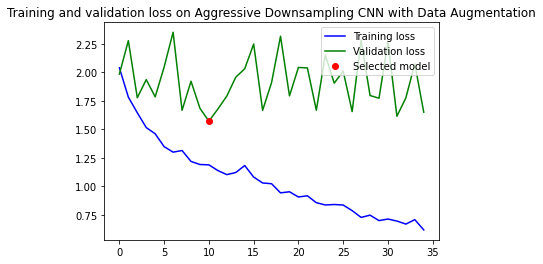
\includegraphics[width=0.9\linewidth]{img/scratch/data_augmented_ad_loss.png}
		\caption{Bigger CNN with aggressive downsampling and data augmentation loss}
		\label{fig:DataAugmentedrAggressiveDownsamplingloss}
	\end{subfigure}
\end{figure}

\medskip 

\noindent Also this time data augmentation did not help, the training loss convergence is smoother and slower but validation curves are very noisy and fang-shaped, showing very bad results and in some iterations almost random predictions. We should increase the network and use some regularization technique like L1 or L2 regularization, but again we cannot train from scratch a network bigger than this one in a reasonable time due to Colab limitations.




\subsection{Inception Blocks}
Inception modules are special convolutional blocks in which we do not define just one layer, but we concatenate more layers with different kernel sizes, together with a max pooling. The idea is that choosing which specific filter to use at each convolutional layer is an hyper-parameter, so it can be source of losses of performance. On the contrary, horizontally concatenating such layers we let the network "learn and decide" which one to use in order to minimize its training loss. Google started exploiting inception modules from GoogleNet(2014), and a finer version of them is present in the modern Inceptionv3 and Inceptionv4. In this section, we try to design and train a Convolutional Neural network equipped with Inception Layers, and we are going to measure its accuracy. 

\subsubsection{Standard CNN with Inception Layers}
In this paragraph we build a model like the 3.1.1 one, but that also exploits custom-defined inception modules. At every module, the network can decide if to use a 3x3 or 5x5 convolution, or a 3x3 max-pooling with stride 1.
The architecture is the following:


\begin{figure}[H]
	\centering
	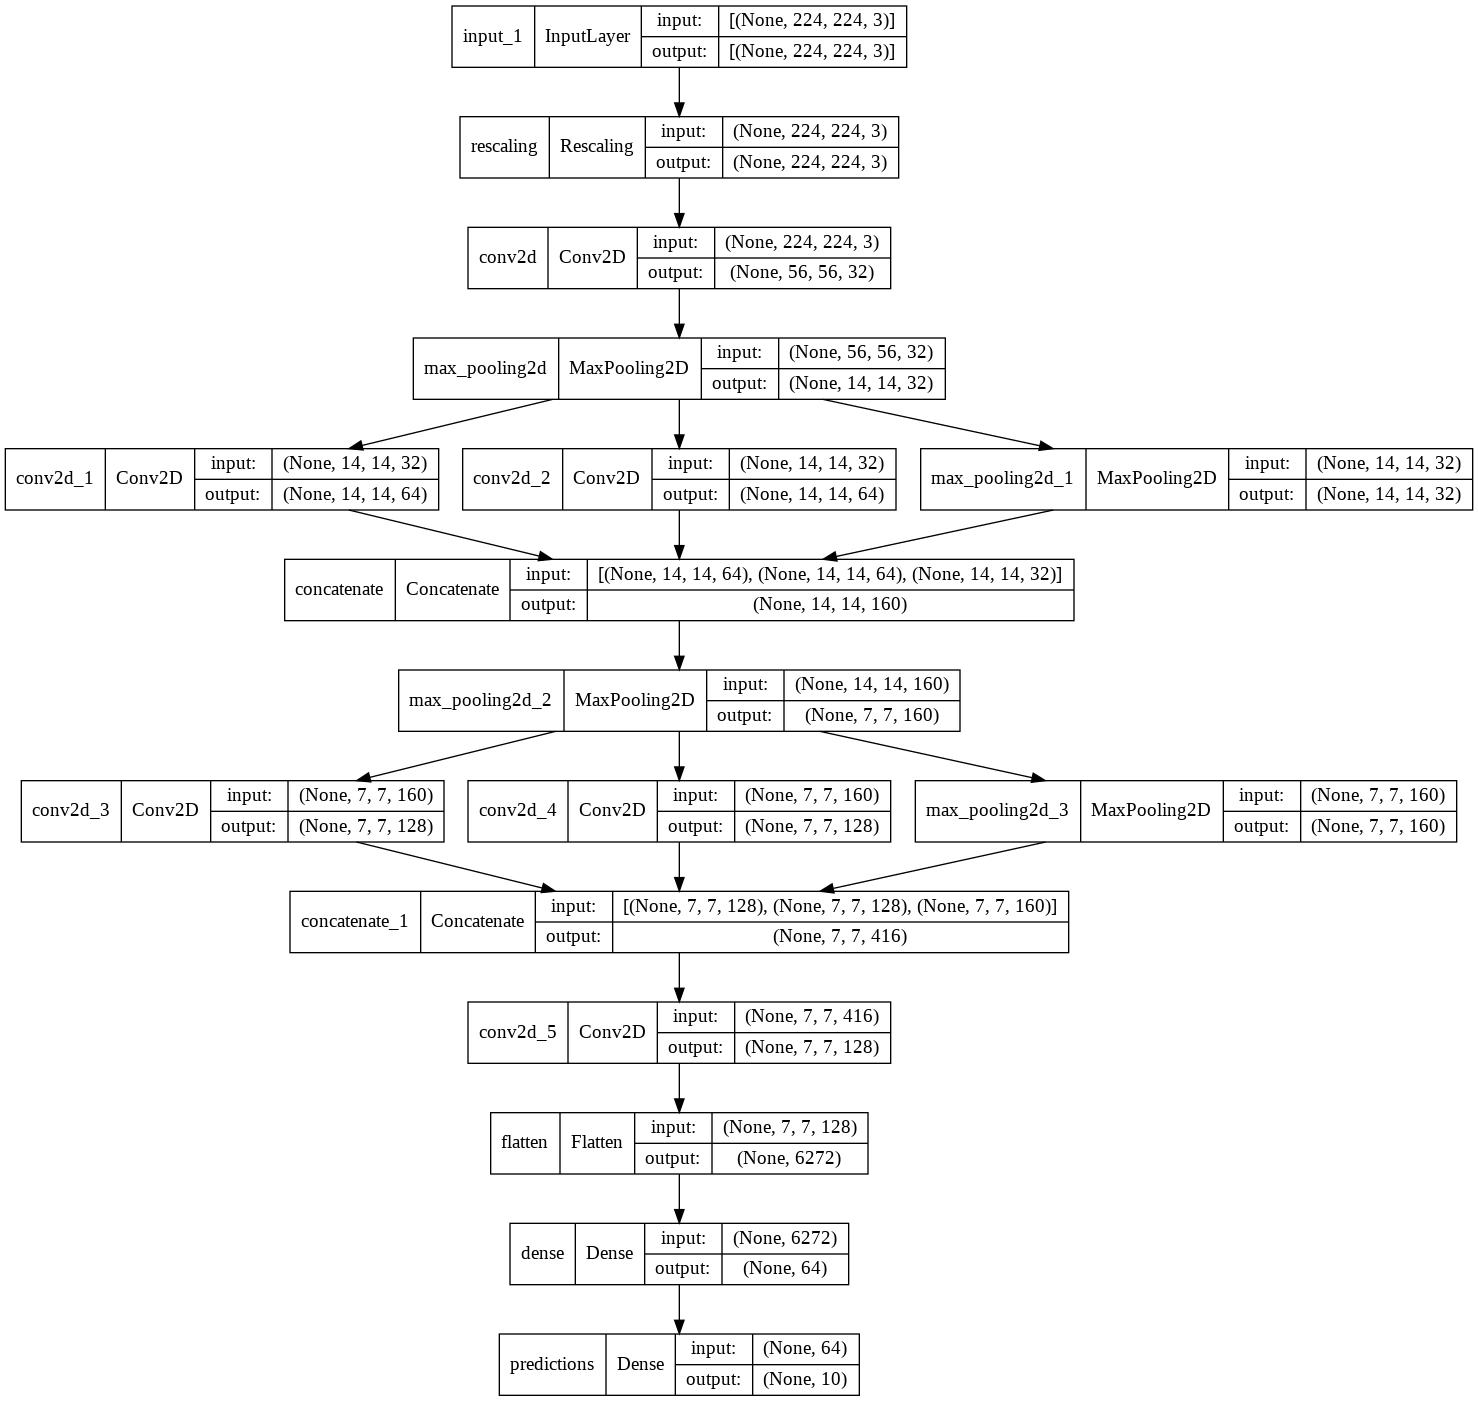
\includegraphics[height=0.8\textwidth]{img/scratch/inception_layers.jpg}
	\caption{CNN architecture with Inception Layers}
	\label{fig:InceptionLayersCNN}
\end{figure}

\medskip

\begin{tabular}{ |p{2cm}|p{2cm}|p{2cm}|p{2cm}|p{2cm}|  }
\hline
\multicolumn{5}{|c|}{CNN with Inception Layers} \\
\hline
\textbf{Epoch stopped} & \textbf{Validation Accuracy} & \textbf{Test Accuracy} & \textbf{Validation Loss} & \textbf{Test Loss} \\
\hline
30 & 0.652 & 0.6915 & 1.1157 & 0.8206\\
\hline
\end{tabular}

\medskip


\begin{figure}[H]
	\begin{subfigure}{0.5\textwidth}
		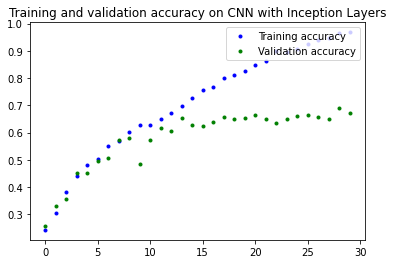
\includegraphics[width=0.9\linewidth]{img/scratch/inception_layer_acc.png} 
		\caption{CNN with inception layers accuracy}
		\label{fig:InceptionLayeracc}
	\end{subfigure}
	\begin{subfigure}{0.5\textwidth}
		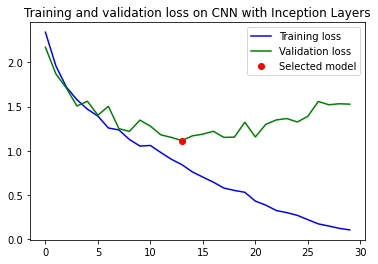
\includegraphics[width=0.9\linewidth]{img/scratch/inception_layer_loss.png}
		\caption{CNN with inception layers loss}
		\label{fig:InceptionLayerloss}
	\end{subfigure}
\end{figure}

\medskip

\noindent The network performed really well, showing quite good accuracy on validation set and great results on test set, both comparable with the ones reached by the 3.2.1 but overcoming the missed convergency problem. 


\subsubsection{Larger CNN with Inception Layers}
In this experiment we try to increase the number of hidden neurons in the fully connected layers and we measure the resulting accuracy. This approach is usually exploited when there is underfitting: in our case there is not. However to increment the size of the dense layer turned out to be very effective in the previous experiments, so we will try to do that, but of course mitigating with dropout to avoid overfitting:

\begin{figure}[H]
	\centering
	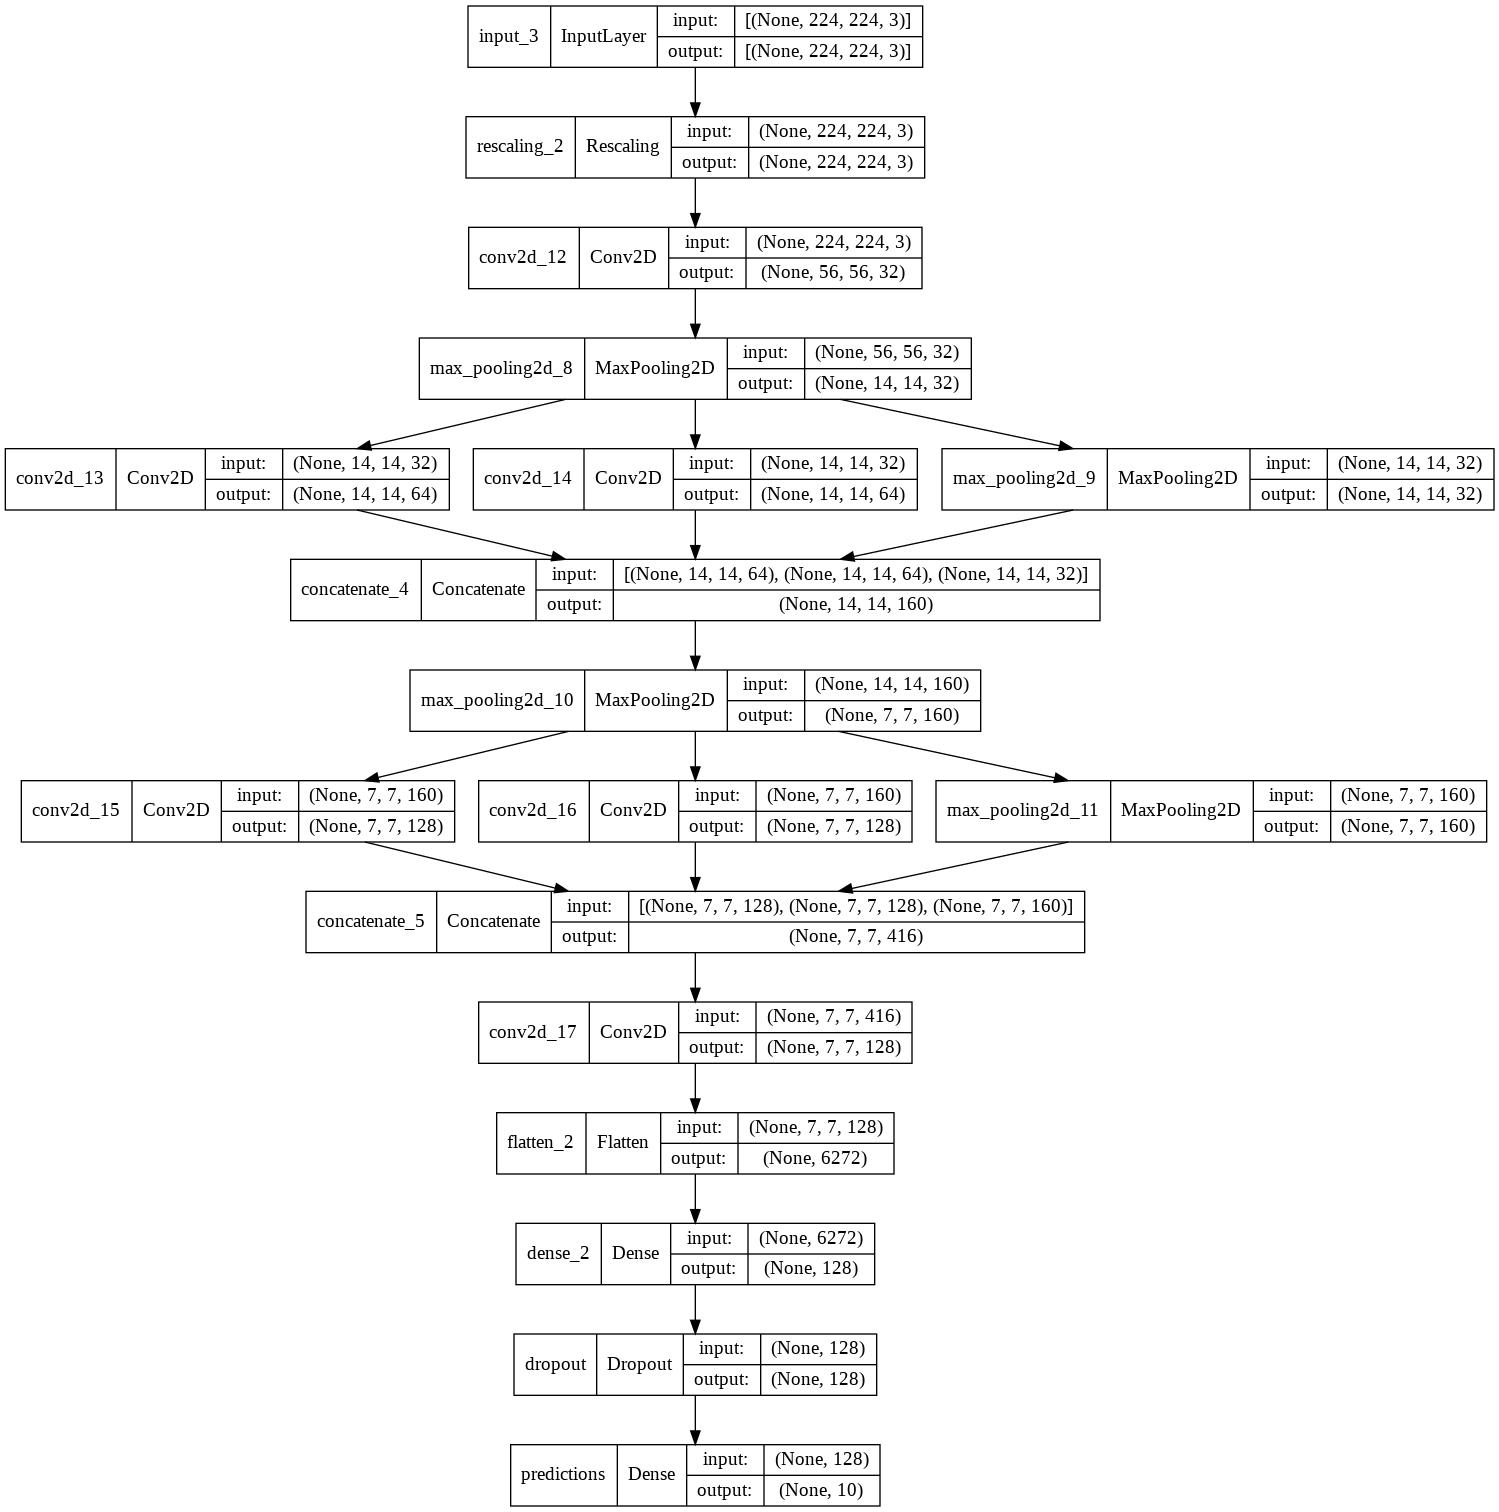
\includegraphics[height=0.8\textwidth]{img/scratch/larger_inception_layers.jpg}
	\caption{Bigger CNN architecture with Inception Layers}
	\label{fig: LargerInceptionLayersCNN}
\end{figure}

\noindent Number of parameters is pretty high, more than 2 millions. The training outcome is the following:

\medskip

\begin{tabular}{ |p{2cm}|p{2cm}|p{2cm}|p{2cm}|p{2cm}|  }
\hline
\multicolumn{5}{|c|}{Bigger CNN with Inception Layers} \\
\hline
\textbf{Epoch stopped} & \textbf{Validation Accuracy} & \textbf{Test Accuracy} & \textbf{Validation Loss} & \textbf{Test Loss} \\
\hline
25 & 0.677 & 0.6219 & 0.9961 & 1.1133\\
\hline
\end{tabular}

\medskip


\begin{figure}[H]
	\begin{subfigure}{0.5\textwidth}
		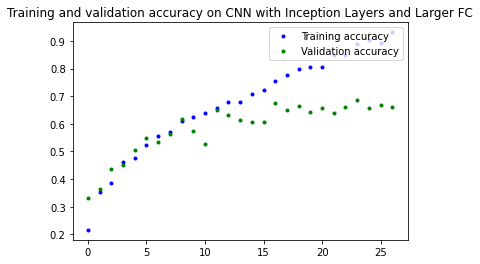
\includegraphics[width=0.9\linewidth]{img/scratch/larger_il_acc.png} 
		\caption{Bigger CNN with Inception Layers accuracy}
		\label{fig:BiggerInceptionLayeracc}
	\end{subfigure}
	\begin{subfigure}{0.5\textwidth}
		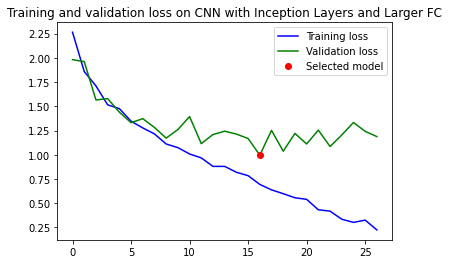
\includegraphics[width=0.9\linewidth]{img/scratch/larger_il_loss.png}
		\caption{Bigger CNN with inception layers loss}
		\label{fig:BiggerInceptionLayerloss}
	\end{subfigure}
\end{figure}

\medskip

\noindent Performances are more or less the same w.r.t. the previous model. Accuracy on validation set is slightly worse but loss is lower, which individuates more "confident", thus robust, predictions on this set. On test set results are not so good as the previous experiment.

\subsection{Hyper-parameters optimization}
Once we found the results of several experiments, we would like to run a hyper-parameter optimization algorithm on the best models found so far, in order to try to tune them to reach even better accuracies in a more stable manner. As we know, there are several algorithms with different complexities and efficiencies, among them we can list Grid Search, Random Search, Bayesian Model and Hyperband. The latter has been chosen to perform our hyper-parameters optimization: hyperband is an algorithm that relies on a principled early-stopping strategy to allocate resources, allowing it to evaluate orders-of-magnitude more configurations than black-box procedures like Bayesian optimization methods.\footnote{LI, Lisha, et al. Hyperband: A novel bandit-based approach to hyperparameter optimization. The Journal of Machine Learning Research, 2017, 18.1: 6765-6816.}
Hyperband is based on the Successive Halving algorithm, which starts from a budget $B$ (e.g. total training epochs or training time ore GPU memory) and a value $n$ of different configurations and at each iteration it discards the worst half. In successive halving, a difficult task is to choose $B$ but more important to choose $n$: the trade-off is between $n$ (that will act as exploration value) and $B/n$ (that will act as exploitation value).
Hyperbands overcomes the problem allocating several combinations of $n$ and $B/n$, keeping $B$ constant at each call of Successive Halving.
The input parameters to the algorithm were:
\begin{itemize}
\item Models: 3.2.2 and 3.3.1 that were 2 of the most performant ones we trained from scratch
\item $R$=20. Because those 2 models needed less than 20 epochs to be trained, this can be a good upper bound for training
\item $\eta$=3 as default
\item $s_{max}=\lfloor \log_{\eta} R \rfloor$=2
\item $B=(s_{max}+1)R$=80
\end{itemize}
With this configuration we run Hyperband on the 2 models, aiming at optimizing the following hyper-parameters:
\begin{itemize}
\item $n\_neurons$: Number of neurons in the FC layer, right after the Flatten and before the classification, chosen as integer value between 0 and 256 with a step of 16
\item $dropout\_rate$: Dropout rate in this layer, as float value between 0 and 0.6
\item Activation function in the convolutional layers. Till now we always considered only ReLU (Rectified Linear Unit), now we introduce the possibility to choose also from ELU (Explonential Linear Unit) or GELU (Gaussian Error Linear Unit)
\item $lr$: Initial Learning rate for the optimizer. Till now we always used default one for ADAM (1e-3), now the tuner will choose a float value between 5e-5 and 5e-3
\end{itemize}
The actual Hyperband optimization we used is the Keras Tuner, which provides automatic APIs to run Hyperband and other algorithms in avery fast and easy way, however consuming much GPU memory and computational time to find the best model. After running the tuner, we saved best models into 2 files and we visualized the best combinations of hyper-parameters, which are:
\begin{itemize}
\item First model: $n\_neurons$=208, $dropout\_rate$=0.03 activation=ReLU, $lr$=0.0012
\item Second model: $n\_neurons$=176, $dropout\_rate$=0.09 activation=ReLU, $lr$=0.0004
\end{itemize}

\noindent As we notice, the optimal choice is to adopt a large number of hidden neurons (between 150 and 225), low or no dropout rate, ReLU as activation function and learning rate that is near the default one (1e-3). The models' performance is the following:


\begin{tabular}{ |p{5cm}|p{2cm}|p{2cm}|p{2cm}|p{2cm}|  }
\hline
\multicolumn{5}{|c|}{Performance comparison} \\
\hline
\textbf{Model} & \textbf{Validation Accuracy} & \textbf{Test Accuracy} & \textbf{Validation Loss} & \textbf{Test Loss} \\
\hline
Custom Aggressive Downsampling(3.2.2) & 0.688 & 0.7910 & 1.0349 & 0.6340\\
\hline
Optimized Aggressive Downsampling & 0.6130 & 0.6020 & 1.0670 & 1.2014\\
\hline
Custom CNN with Inception Layers(3.3.1) & 0.652 & 0.6915 & 1.1157 & 0.8206\\
\hline
Optimized CNN with Inception layers & 0.664 & 0.6990 & 0.9695 & 0.9797\\
\hline
\end{tabular}

\medskip 

\noindent Comparing the performance of the models found by the tuner w.r.t their original counterparts, we actually observe few differences: the first optimized model is slightly less performant than the custom one, while the optimized CNN with Inception Layers achieved slightly better results, but on test set it didn't overcome the loss value of the other model.

\subsection{Visualization techniques}
In this chapter we will adopt some technique to visually analyze what the network focuses on, in order to understand if our CNN is robust and is looking to the correct features to recognize the author of each painting. Taking again the 3.2.2 and 3.3.1 models, we will evaluate:
\begin{itemize}
\item The heatmap of class activations, that is starting from the activation level of a certain layer of our network with respect to a specific class, we apply a weighted gradient to highlight in the input image what portions of it were considered the most in order to classify the image with that label\footnote{SELVARAJU, Ramprasaath R., et al. Grad-cam: Visual explanations from deep networks via gradient-based localization. In: Proceedings of the IEEE international conference on computer vision. 2017. p. 618-626.}
\item A partial exclusion mask, that is we try to occlude different portions and positions of the input image, to understand if the network is still able to classify it correctly
\end{itemize} 

\subsubsection{Class activations heatmap}
The idea is, given an input of the correct class, to map the gradients of the top-predicted class w.r.t. the activations of the convolutional layer we are analyzing, and then superimpose this heatmap to the input in order to understand which portions were mostly important for the final decision.
We took as input image, a test sample of Vincent Van Gogh, which had been correctly classified by the two considered network at testing phase. The image is the following: \ref{fig: Test_image_visualization}


\begin{figure}[H]
	\centering
	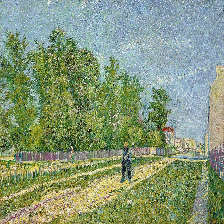
\includegraphics[height=0.6\textwidth]{img/scratch/visualization/test_image.png}
	\caption{Test image}
	\label{fig: Test_image_visualization}
\end{figure}

\noindent Once selected our models, we replace the last layers with new ones in order to observe more clearly what the back-prop gradients are, then after submitting the test image we record the locations of the activation map of the last layer that were "excited" the most. In this way we obtained our heatmap, which can be superimposed to the test image to visualize which locations were considered as more interesting for the monitored convolutional layer. Applying it for the last convolution of both the models we obtained:


\begin{figure}[H]
	\begin{subfigure}{0.5\textwidth}
		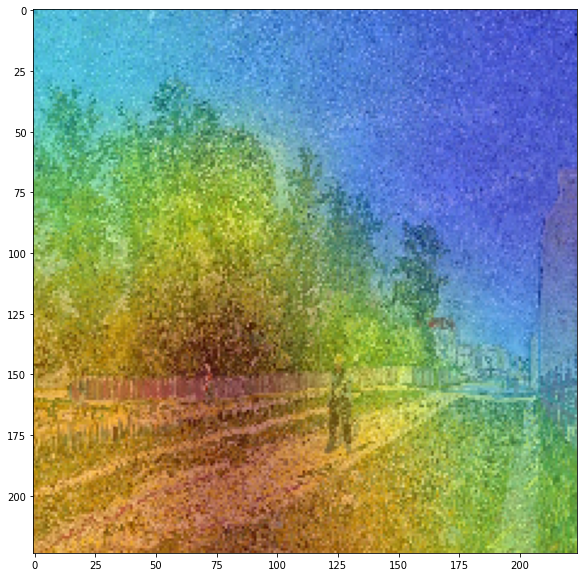
\includegraphics[width=0.9\linewidth]{img/scratch/visualization/ad_heatmap.png} 
		\caption{Class activation map of the last layer of 3.2.2}
		\label{fig:ad_heatmap}
	\end{subfigure}
	\begin{subfigure}{0.5\textwidth}
		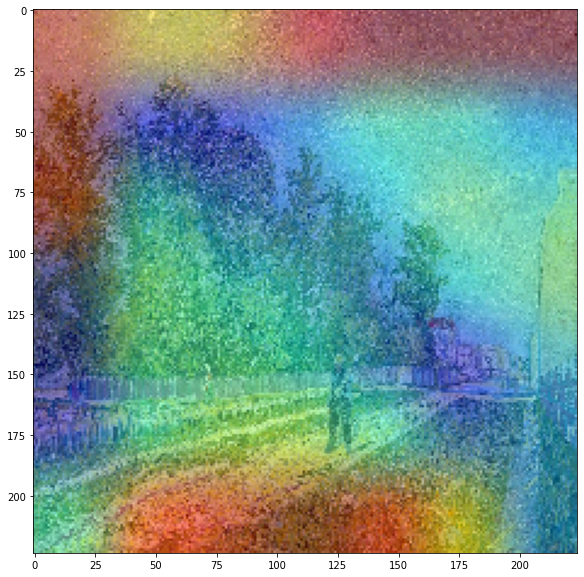
\includegraphics[width=0.9\linewidth]{img/scratch/visualization/il_heatmap.png}
		\caption{Class activation map of the last layer of 3.3.1}
		\label{fig:il_heatmap}
	\end{subfigure}
\end{figure}

\noindent As we can see, the first model tends to look more "at the center" of the image, maybe seeking for author's typical characters/objects, or maybe recognizing the style or the typical color pattern of the objects. Remember also that this network aggressively downsamples the input image, thus the remaining information at the center of the image will be very various and precious for this network. On the other hand, the second model seems to "look at the edges", activating the most this heatmap in correspondence of the sky and the road: this network maybe is able to recognize the style of the author, and classifies images, distinguishing how he/she represents common elements and maybe which colors and patterns he/she uses to characterize the background.

\subsubsection{Occlusion masks}
The idea of occlusion masks is very simple and intuitive: in order to see what portions of the test image are considered to take the decision of the correct class, we "hide" with a black box a part of it and we submit the resulting image to the classifier, annotating the response. Iterating for different positions and different sizes, we can estimate the robustness of the network and the portions of the input image that it considers as "fundamental" to take the correct decision.
We iterated the algorithm with 3 occlusion mask sizes: 10, 28 and 35 pixels; we applied it every size*3 pixels in width and height, and the results are the following:
\begin{itemize}
\item With size=10, 9 masks are produced, both the networks are still able to correctly predict \textit{Vincent Van Gogh} independently from the covered zone
\item With size=35, 4 masks are produced, both the networks miss all prediction, outputting $Rembrandt$
\item With size=28, 4 masks are produced, while the first network is still always able to classify the image as \textit{Vincent Van Gogh}, the second network mispredicts twice.
\end{itemize}

\noindent Applied occlusion masks and relative predictions with size=28 are:

\begin{figure}[H]
	\begin{subfigure}{0.5\textwidth}
		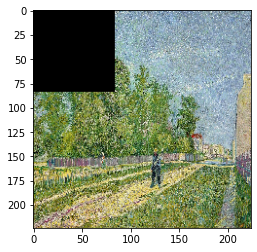
\includegraphics[width=0.9\linewidth]{img/scratch/visualization/occlusion_mask_1.png} 
		\caption{Vincent Van Gogh -- Vincent Van Gogh}
		\label{fig:oc_mask_1}
	\end{subfigure}
	\begin{subfigure}{0.5\textwidth}
		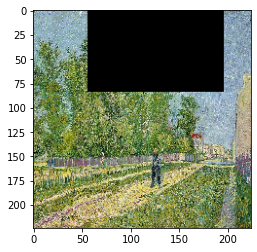
\includegraphics[width=0.9\linewidth]{img/scratch/visualization/occlusion_mask_2.png} 
		\caption{Vincent Van Gogh -- Alfred Sysley}
		\label{fig:oc_mask_2}
	\end{subfigure}
	\begin{subfigure}{0.5\textwidth}
		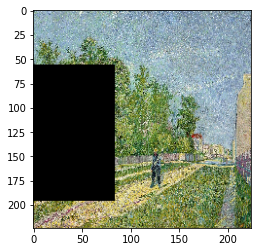
\includegraphics[width=0.9\linewidth]{img/scratch/visualization/occlusion_mask_3.png} 
		\caption{Vincent Van Gogh -- Vincent Van Gogh}
		\label{fig:oc_mask_3}
	\end{subfigure}
	\begin{subfigure}{0.5\textwidth}
		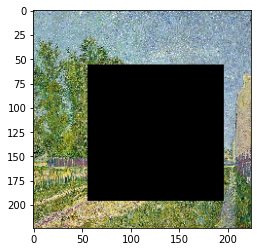
\includegraphics[width=0.9\linewidth]{img/scratch/visualization/occlusion_mask_4.png} 
		\caption{Vincent Van Gogh -- Rembrandt}
		\label{fig:oc_mask_4}
	\end{subfigure}
\end{figure}

\medskip

\noindent From these results we can infer very interesting knowledge. First of all, the 3.2.2 network proved to be very robust and to be able to correctly classifying the image even in the most adverse situation, i.e. when the center is completely covered. This is absolutely not trivial if we consider that, as shown in the 3.5.1 heatmap, it tends to look exactly at the center to classify the painting. Even more interesting what concerns the second model: as we observed in the 3.5.1 heatmap, it tends to focus on background characteristics, especially sky or ground style, and in fact when the sky or the center of the image (including the road) are occluded, the classification is wrong. In spite of it, we can say that it is "not so wrong": the first misprediction (b) outputted \textit{Alfred Sisley}, which was an impressionist (\textit{Van Gogh} was post-impressionist) whose style differs a bit from the Dutch painter, but the biggest differences are actually in the sky which is usually calm and regular for \textit{Sisley}, dramatic for \textit{Van Gogh}; without this information the error is comprehensible. A similar consideration holds for the second misprediction (d): we can argue that from the center of the image the network considers very much the color, and in fact when we substituted the center with a black box, it classified the test image as \textit{Rembrandt}, who is known for very dark paintings, with a lot of black in the center.
Anyway, from those results, the model 3.2.2 showed to be more robust and precise with respect to the 3.3.1 one. 